\chapter{Bài toán và giải pháp}\label{chap:ProblemAndSolve}
		Sau khi phân tích, nghiên cứu các hệ thống và sản phẩm khác thì nhóm đã liệt kê ra một số bài toán cần phải giải quyết. Sau đây là phần trình bày của nhóm.
		
		\section{Bài toán xác thực user}
		Như chúng ta đã biết thì HTTP là 1 giao thức Stateless, nghĩa là khi Client gửi dữ liệu lên Server, Server thực thi xong và trả kết quả về cho Client thì quan hệ giữa Client và Server sẽ bị cắt đứt, Server sẽ không lưu lại bất cứ dữ liệu trạng thái gì của Client. Nói một cách dễ hiểu hơn là khi ta đăng nhập vào MyBK và sau đó di chuyển sang trang Thông tin Sinh viên thì chúng ta phải đăng nhập lại vì Server không lưu giữ bất kì thông tin gì của chúng ta. Để giải quyết vấn đề này thì Session/Cookies ra đời.
		
		\newpage
	
		\begin{figure}[!ht]
			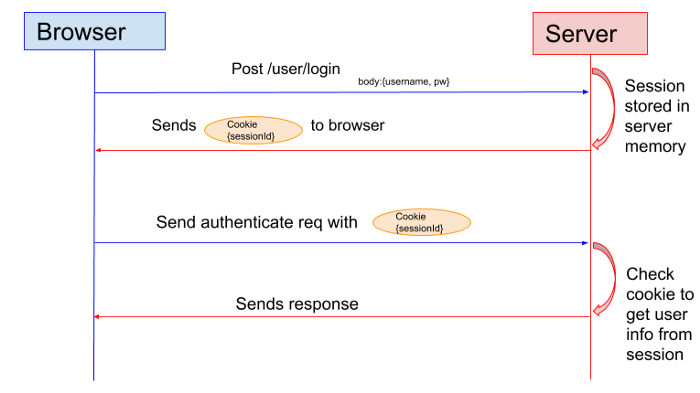
\includegraphics[width=1\textwidth]{Images/session-cookies.png}
			\centering
			\linebreak
			\caption{Xác thực dựa trên Session và Cookies}
		\end{figure}
		
		Đầu tiên user nhập thông tin tài khoản của mình. Sau khi kiểm tra đúng thông tin đăng nhập thì Server sẽ tạo ra 1 sessionID, lưu lại vào Database và trả về cho Client. Sau đó mỗi request gửi lên thì Client sẽ chèn sessionId vào Cookies và gửi lên cho Server từ đó Server kiểm tra và biết được chính xác Client đó là ai.
		
		Đối với hệ thống Micro Service thì việc xác thực theo cách này có 1 vấn đề đó là cần phải có 1 nơi để lưu trữ thông tin về session, ngoài ra cần phải xử lý các session đã hết hạn. Việc này có thể là giảm hiệu năng của 1 hệ thống Micro Service.
		
		Sau khi tìm hiểu thì nhóm sử dụng cơ chế xác thực dựa trên token. Với cơ chế như sau:
		
		\newpage
		
		\begin{figure}[!ht]
			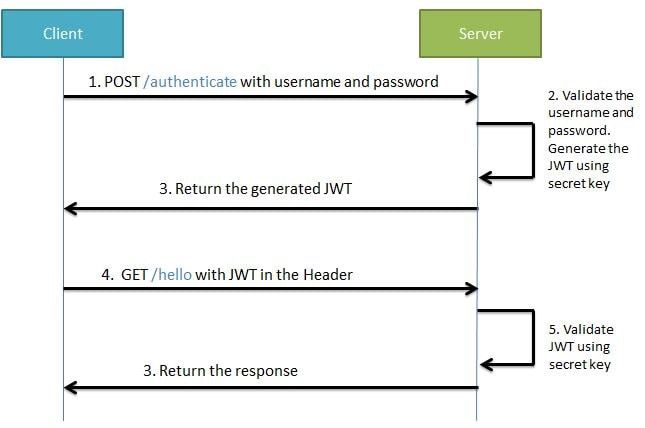
\includegraphics[width=1\textwidth]{Images/authbasedtoken.jpg}
			\centering
			\linebreak
			\caption{Xác thực dựa trên token}
		\end{figure}
		
		\begin{itemize}
                \item Client gửi thông tin đăng nhập lên Server
                \item Server xác thực thông tin đăng nhập. Nếu đúng sẽ tạo ra 1 token và gửi về cho Client
                \item Client đính kèm token mỗi khi request lên Server 
            \end{itemize}
		
		
		\section{Bài toán xác thực giữa các service}
		Do các service đươc deploy trên môi trường mạng vì thế có thể tiểm ẩn nhiều rủi ro bảo mật khi có sự giao tiếp giữa các service với nhau. Một kẻ tấn công nào đó có thể giả danh và gửi các request lên cho service của hệ thống xử lý. Do đó kẻ tấn công có thể lấy được các thông tin nhạy cảm của user (như số điện thọai, tên, địa chỉ, ngày tháng năm sinh, ...). Đây là một điều rất cấm kỵ khi chúng ta phải có nghĩa vụ bảo mật các thông tin nhạy cảm cho user.\\
		
		Sau khi tìm hiểu và so sánh các phương pháp thì nhóm sử dụng phương pháp tạo chữ ký số để xác thực request giữa các service với nhau. Khi service A muốn gọi service B thì service A phải có key của service B, Service A sẽ gửi thêm 1 trường thông tin là \textbf{sig = SHA256(data + key)}, service B khi nhận request thì sẽ tạo sig dựa vào key của mình và so sánh 2 sig đó có giống nhau không. Nếu giống thì mới tiếp tục thực hiện request của Service A, còn nếu không thì sẽ trả về lỗi cho service A.
		
		
		\section{Bài toán nhận nhiều Request của User}
		Thông thường 1 request của User sẽ được xử lý như sau: 
		    \begin{itemize}
                \item User gửi Request lên Server
                \item Server xử lý
                \item User nhận Response về từ Server 
            \end{itemize}
        Trong quá trình chờ Server xử lý thì User sẽ phải chờ đợi và nếu quá trình xử lý diễn ra lâu (bởi vì Server phải lưu thông tin vào database hay phải gọi Server khác,...) chính điều này sẽ ảnh hưởng đến trải nghiệm của User.\\
        Ngoài ra, trong những khoảng thời gian diễn ra các chương trình khuyến mãi giảm chi phí vận chuyển hoặc trong thời gian dịch bệnh thì nhu cầu vận chuyển hàng hóa để đáp ứng như cầu tiêu thụ của người dân. Do đó có thể trong 1 khoảng thời gian ngắn lượng Request đến hệ thống tăng cao. Nếu vẫn xử lý với cơ chế như bình thường thì hệ thống sẽ chết hoăc có thể không nhận đươc Request của User nữa. Điều này cũng ảnh hưởng nghiêm trọng đến trải nghiệm của User.\\
        Sau khi tìm hiểu và phân tích thì nhóm hiện thực chức năng tạo đơn hàng bằng cơ chế bất đồng bộ như sau:\\
        
        \begin{figure}[!ht]
			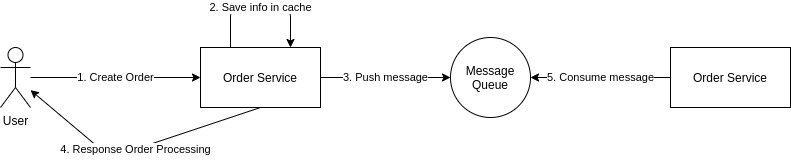
\includegraphics[width=1\textwidth]{Images/problem1.jpg}
			\centering
			\linebreak
			\caption{Quá trình tạo đơn hàng}
		\end{figure}
        
        Ở đây nhóm sử dụng MessageQueue(ActiveMQ) để hiện thực cơ chế bất đồng bộ. Sau khi user thực hiện tạo đơn hàng thì hệ thống sẽ lưu thông tin đơn hàng đó vào Cache, sau khi đã lưu thông tin đơn hàng vào Cache thì ta ngay lập tức phản hồi về cho User là đơn hàng đang được xử lý. Tiếp theo ta push message tạo đơn hàng đó vào MessageQueue, và sau đó đơn hàng sẽ được consume và tiếp tục xử lý.\\
        Việc sử dụng MessageQueue làm tách rời quá trình xử lý, Producer (service push message) chỉ cần đẩy message lên mà không cần quan tâm là message đó đã được xử lý hay không và Consumer (service consume message) chỉ cần lấy message và xử lý. Các mesage sẽ được lưu trữ trong Queue và chỉ mất đi khi đươc consume, điều này đảm bảo tất cả các message đề đươc xử lý duy nhất 1 lần và tất cả message sẽ không mất đi ngày cả khi OrderService bị chết do sự cố nào đó. Và đặc biệt lợi ích cuối cùng đó là trải nghiệm của User, User sẽ nhận phản hồi gần như lập tức sau khi tạo đơn hàng (mặc dù đơn hàng vẫn đang tiếp tục đươc xử lý) mà không cần phải chờ đợi các bước xử lý mất thời gian ở phía sau. 
	
		\section{Bài toán giảm thời gian xử lý khi User truy xuất thông tin}
		    Trong quá trình sử dụng ứng dụng thì việc lấy và hiện thị thông tin ra cho User diễn ra rất thường xuyên. Thông thường quá trình đó diễn ra như sau:
		    \begin{itemize}
                \item User gửi Request lấy thông tin lên Server
                \item Server truy xuất vào Database
                \item User nhận Response về từ Server 
            \end{itemize}
            
            
            Ở đây viêc truy xuất vào Database thường xuyên có thể làm giảm thời gian phản hồi do phải thực thi nhiều I/O operation. \\
            Vì thế, sau khi tìm hiểu và nghiên cứu thì nhóm sẽ sử dụng Cache để lưu lại các thông tin mà user thường xuyên truy xuất trong memory. Do thông tin được lưu trữ trong memory nên việc truy xuất và lấy các thông tin đó đươc thực hiện rất nhanh (gấp 500 lần so với thông tin lấy từ Database). Có rất nhiều chiến lược Cache có thể sử dụng nhưng nhóm sử dụng chiến lược Cache Aside để phù hợp với nhu cầu của ứng dụng:
            
            \begin{figure}[!ht]
			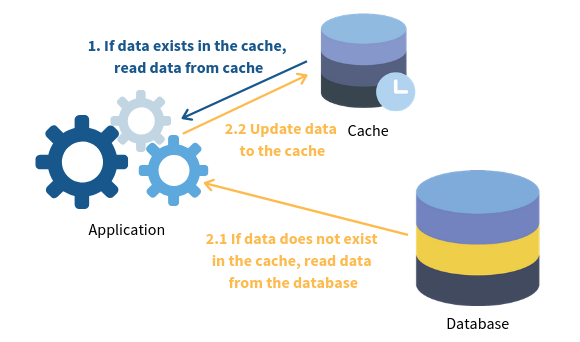
\includegraphics[width=1\textwidth]{Images/problem2.png}
			\centering
			\linebreak
			\caption{Chiến lươc Cache Aside}
	       	\end{figure}
	       	
	        Đầu tiên khi muốn lấy thông tin nào đó thì ta tiến hành tìm trong Cache. Nếu trong Cache có thông tin cần tìm kiếm thì lập tức trả thông tin đó về cho User, nếu không tìm thấy trong Cache thì ta tiến hành tìm kiếm trong Database, sau đó lưu thông tin đó vào Cache rồi mới trả về cho User.\\
	        Việc sử dụng Cache đem lại hiệu quả nhưng cũng có 1 số điểm cần lưu ý như:
	         \begin{itemize}
                \item Thứ nhất là \textbf{Stale Cache}: Có nghĩa là dữ liệu trong Database và trong Cache không nhất quán với nhau dẫn đến trả về các thông tin cũ cho User. Nhóm giải quyết vấn đề này bằng cách mỗi khi cập nhật lại thông tin trong Database thì đều cập nhật luôn thông tin trong Cache. Việc này có thể làm tốn thêm nhiều chi phí nhưng nhóm chỉ lưu các thông tin mà User thường xuyên truy xuât nên chi phí sẽ giảm bớt và rất xứng đáng so với hiệu quả to lớn mà Cache mang lại.
                \item Thứ hai là \textbf{Invalidate Cache}: Có nghĩa là nếu để Cache quá lâu trong memory thì sẽ gây tiêu tốn dung lượng, còn nếu để Cache quá nhanh thì sẽ không có hiệu quả do cứ phải truy xuất Database nhiều. Trong quá trình tìm hiểu và thử nghiệm thì nhóm đã thiết lập thời gian tồn tại trong memory là 30 ngày. Là con số có thể chấp nhận đươc đối với mỗi đơn hàng mà User tạo ra.
            \end{itemize}
            
        
			
		\section{Bài toán xác định kho nguồn - kho đích ngắn nhất và tính chi phí vận chuyển}
			Để doanh nghiệp có thể tiết kiệm chí phí cũng như giảm được chí phí vận chuyển cho khách hàng thì bái toán xác định kho nguồn - kho đích so với địa chỉ của người gửi - người nhận sao cho ngắn nhất là một bài toán cần phải giải quyết sao cho tối ưu.\\\\
			\indent	Để xác định kho nguồn - kho đích ngắn nhất nhóm đã tìm quảng đường vận chuyển ngắn nhất giữa địa chỉ của người gửi so với tất cả địa chỉ của kho nguồn và giữa địa chỉ của người nhận so với tất cả địa chỉ của kho đích. Để xác định được quãng đường (km) nhóm đã sử dụng Google Map API để có thể tính đường quãng đường giữa hai địa chỉ cần xác định. Từ đó nhóm đã tìm được quãng đường tối ưu ngắn nhất và sử dụng tổng quãng đường vẫn chuyển ngắn nhất giữa hai địa chỉ người gửi - người nhận để tính toán chi phí cần vận chuyển đơn hàng cho người gửi. 
		\section{Bài toán thanh toán chi phí vận chuyển} 
		Thông thường để thanh toán chi phí vận chuyển thì người dùng sử dụng phương thức thu hộ (COD) hoặc thanh toán bằng tiền mặt khi nhận hàng, điều này gây ra nhiều bất tiện cho người dùng. Vì vậy, với xu hướng thanh toán không tiền mặt đang phát triển rộng rãi như hiện nay nên nhóm đẵ bắp kịp xu thế tích hợp cổng thanh toán online ZaloPay để người dùng có thể sử dụng thanh toán qua 3 hình thức thanh toán ví ZaloPay, Visa, Master, JCB (qua Cổng ZaloPay), thẻ ATM (qua Cổng ZaloPay).
		
		\begin{figure}[!ht]
			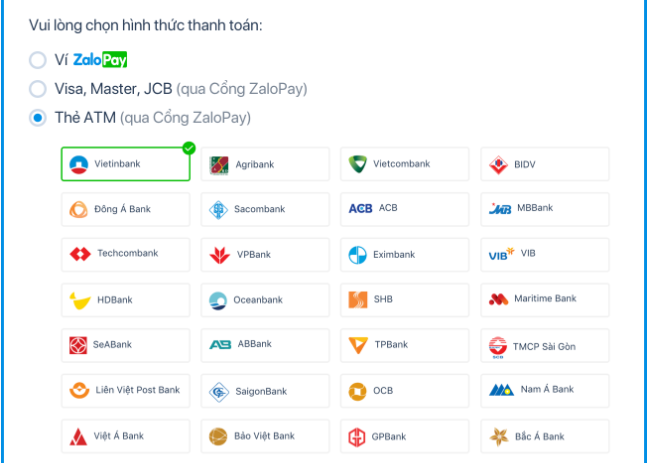
\includegraphics[width=1\textwidth]{Images/payment.png}
			\centering
			\linebreak
			\caption{Hình thức thanh toán}
		\end{figure}
		\section{Bài toán phân phối đơn hàng cho tài xế }
		    Trong các ứng dụng vận chuyển hàng thì bái toán phân phối là một bài toán rất hay, việc giải quyết bài toán này sao cho tối ưu có ảnh hưởng không nhỏ đến doanh thu của doanh nghiệp cũng như là chi phí của khách hàng.\\
		    Ở hệ thống vận chuyển liên tỉnh mà nhóm đang làm thì sẽ có 3 giai đoạn phân phối: Đầu tiên là phân phối đơn hàng cho tài xế đi lấy, tiếp theo là phân phối đơn hàng cho tài xế liên tỉnh, cúôi cùng là phân phôi đơn hàng cho tài xế đi giao.
		    
		     \begin{itemize}
                \item \textbf{Phân phối đơn hàng cho tài xế đi lấy:} Sau khi đơn hàng được tạo ra bởi user thì sẽ có 2 cách để nhận hàng. Thứ nhất là user sẽ trưc tiếp đem hàng đến kho, thứ hai là hệ thống sẽ gán đơn đó cho tài xế và tài xế sẽ đi lấy hàng. Ở đây chúng ta nói về cách thứ hai. Sau khi đơn hàng được tạo ra thì hệ thống sẽ xác định được con đường ngắn nhất giữa 2 kho là kho nguồn và kho đích. Tài xế đi lấy sẽ là nhân viên ở kho nguồn. Hệ thống sẽ ngẫu nhiên thông báo cho một số tài xế ở kho nguồn là có đơn cần lấy. Tài xế nào đống ý nhận đơn trước thì sẽ được ưu tiên đi lấy hàng trước.\\
                Do hàng vận chuyển liên tỉnh, có thể số lượng sẽ rất lớn vì vậy nếu tài xế đầu tiên không lây hết thì hệ thống sẽ tự động thông báo cho các tài xế tiếp theo. Cứ như vậy đến khi hàng được lấy hết và chở về kho nguồn.\\
                Ở đây hệ thống sẽ thông báo cho một số tài xế của kho nguồn nhằm hạn chế việc tài xế được thông báo nhưng đang bận và chưa thể vận chuyển hàng về kho ngay lập tức được. Điều đó có thể làm chậm trễ thời gian giao vận mà user mong muốn gây ảnh hưởng đến trải nghiệm của user.
            
                \item \textbf{Phân phối đơn hàng cho tài xế  liên tỉnh:} Sau khi đơn hàng được vận chuyển đến kho nguồn thì việc tiếp theo hệ thống sẽ gán đơn hàng đó cho tài xế liên tỉnh để vận hàng hàng đến kho đích.\\
                
                Việc gán liên tỉnh sẽ được thực hiện vào 1 khung giờ cố định trong ngày (ví dụ: 19h mỗi ngày) và sẽ gán đơn hàng lên xe của 1 tài xế đến khi xe đầy thì chuyển sang xe của tài xế khác.\\
                
                Viêc gán vào 1 khung giờ cố định trong ngày nhằm để không làm giảm hiệu năng của hệ thống bời vì việc gán tài xế sẽ phải gọi service khác để lây thông tin và lưu database. Việc gán đơn hàng cho 1 xe đến khi đầy nhằm hạn chế tối đa chi phí bỏ ra để vận chuyển các đơn hàng đó. Nếu cùng 1 số lượng đơn hàng nhưng được gán lên rất nhiều xe để vận chuyển liên tỉnh thì sẽ tốn chi phí rất nhiều.
                
                \item \textbf{Phân phối đơn hàng cho tài xế  đi giao:} Sau khi đến kho đích thì đơn hàng tiếp tục được gán cho tài xế của kho đích đi giao. Việc gán đơn cho tài xế đi giao cũng được thực hiện vào 1 khung giờ cố định trong ngày và cách gán là lấy ra tất cả tải xế đi giao của kho đích và gán đều các đơn hàng cho tất cả tài xế. Việc gán này nhằm đảm bảo thời gian nhận hàng của người nhận là nhanh nhất có thể.
                
            \end{itemize}
            
            
            \section{Bài toán lưu trữ và truy xuất dữ liệu thống kê}
                Trong quá trình hoạt động và vận hành của hệ thống thì user thường xuyên xem lại những lịch sử mua hàng hay quản lý cần thống kê lượng tiền, lượng giao dịch xảy ra trong một khoảng thời gian nào đó.\\
                Thông thường chúng ta sẽ lưu hết vào Database rồi query SELECT COUNT(*) WHERE STARTDATE<=Date AND Date<=ENDDATE. Việc query như vậy vào Database sẽ được xử lý rất lâu cho nên sẽ làm giảm trải nghiệm của user.\\
                Sau khi tìm hiểu và nghiên cứu thì nhóm sử dụng cấu trúc dữ liệu \textbf{HyperLoglog} được hỗ trợ bởi Redis nhằm lưu trữ dữ liệu thống kế để mỗi khi cần chúng ta có thể truy xuất trong nháy mắt.\\
                \textbf{HyperLoglog} giúp chúng ta tính gần đúng các giá trị khác nhau trong tập hợp, thuật toán này có độ chính xác cao mà vẫn giữ được dung lượng dữ liệu rất bé, hỗ trợ nhiều thao tác liên quan tới việc đếm 1 phần tử trong 1 hoặc nhiều tập hợp. Và quan trọng nhất là nó rất nhanh nêu chúng ta tổ chức dữ liệu một cách hợp lý.\\
                
                \begin{figure}[!ht]
			    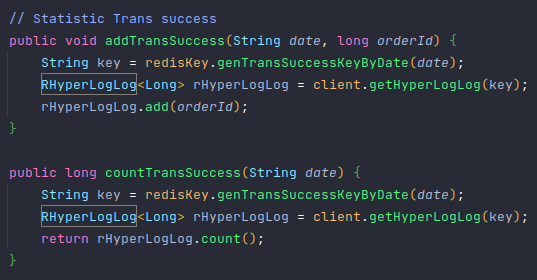
\includegraphics[width=1\textwidth]{Images/hyperloglog.png}
			    \centering
			    \linebreak
			    \caption{Ví dụ về HyperLoglog}
	       	    \end{figure}
	       	
	       	    Trong đoạn code trên ta lưu thông tin của số giao dịch thành công trong 1 ngày. Khi có yêu cầu lấy thông tin về số giao dịch thành công trong một khoảng thời gian nào đó thì ta chỉ cần gọi hàm như ví dụ để lấy. Do các thông tin này được lưu trên memory nên việc xử lý rất nhanh đảm bảo trải nghiệm tốt cho user.
		  
		  \section{Bài toán triển khai các services và cơ sở hạ tầng}
		 
		  
		  Việc deploy hệ thống có thể được hỗ trợ bởi rất nhiều bên như: Git, Heroku, ... thông thường chúng ta chỉ đưa mã nguồn lên Git, thiết lập một vài bước là có thể dễ dàng triển khai hệ thống lên cho khách hàng sử dụng. Nhưng do nhóm sử dụng khá nhiều hạ tầng liên quan để tăng cường hiệu suất cho hệ thống như: Redis, Kafka, Mysql, Message Queue, Cassandra, ...cho nên việc sử dụng các nền tảng đó sẽ không được hỗ trợ một cách tối đa. Ngoài ra để hiểu rõ hơn về quy trình deploy một ứng dụng cũng như là cơ hội để có thể áp dụng các kiến thức đã được học về Network, System, Security, ... vào thực tế thì nhóm quyết định thuê 1 VPS (Virtual Private Server) trên Google Cloud Platform để tự cấu hình và triển khai hệ thống của mình.
		  
		  Như đã trình bày ở phần Công nghệ để deploy nhanh chóng, tiện lợi các services và cơ sở hạ tầng đi kèm thì nhóm sử dụng nền tảng \textbf{Docker} và \textbf{Docker compose}.
		  
		  
		  \begin{figure}
		  	\centering
		  	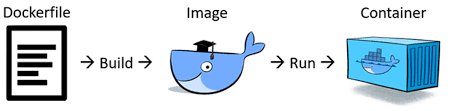
\includegraphics[width=0.8\linewidth]{Images/flowDocker}
		  	\linebreak
		  	\caption{Flow docker}
		  \end{figure}
		  
		  Đầu tiên thì mỗi service cần phải có một \textbf{Dockerfile}, sau đó tiến hàng build Dockerfile thì ta có được \textbf{Image}, cuối cùng chỉ cần chạy Image đó là ta đã deploy được service trong \textbf{Container}.
		  
		  \begin{figure}
		  	\centering
		  	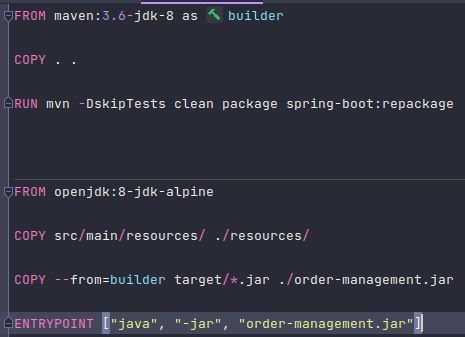
\includegraphics[width=0.7\linewidth]{Images/DockerfileOrderService}
		  	\linebreak
		  	\caption{Dockerfile OrderService}
		  \end{figure}
	  \newpage
		  
		  Dockerfile thực thi các câu lệnh để build ra file *.jar và chạy file jar đó trong containers. Ở đây thì nhóm có tìm hiểu một số kỹ thuật để tăng cường hiệu suất cho Docker như sau:
		  
		  \begin{itemize}
		  	\item \textbf{Multi-stage build}: Thông thường để chạy được service ta cần phải tạo môi trường, cấu hình package, module, ... và sẽ cần dung lượng khá cao, làm cho Image nặng lên từ đó làm tăng thời gian build, run và làm giảm hiệu suất của Docker. Vì thể nhóm sẽ build Image trên 2 stage, ở stage thứ nhất thì ta thiết lập môi trường, các package liên quan sau đó tiến hành build file *.jar. Ở stage thứ 2 ta chỉ cần copy file *.jar qua và thực thi. Điều này giúp cho quá trình build và run Image trở nên nhanh hơn đáng kể.
		  	\item \textbf{Sử dụng base image đươc dựng trên alpine}: Alpine Linux là một distro linux dựa trên musl và busybox, được phát triển chú trọng về đơn giản, bảo mật và hiệu quả tài nguyên. Ở đây nhóm đã sử dụng base image đó là: openjdk:8-jdk-alpine để thực thi file *.jar.
		  \end{itemize}
		  
		  
		  Một hệ thống thông thường sẽ phải deploy rất nhiều container khác nhau. Khi có nhiều container việc phải start, stop, run từng container trở nên khó khăn và khó quản lý. Vì thế nhóm đã dụng \textbf{Docker compose} cho phép quản lý nhiều container một cách rất dễ dàng.
		  
		  Tương tự như các service thì các cơ sở hạ tầng như: MySQL, Cassandra, Redis, Kafka, ActiveMq, ... cũng được deploy và triển khai dựa trên Docker.
		  
		  
		  
		  \begin{figure}
		  	\centering
		  	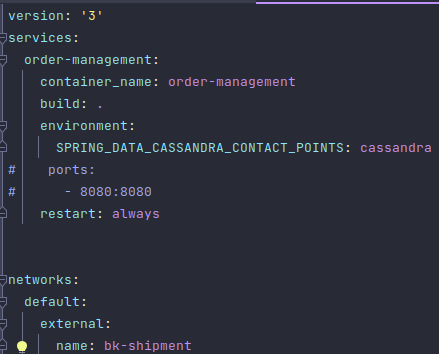
\includegraphics[width=0.8\linewidth]{Images/DockercomposeOrderService}
		  	\linebreak
		  	\caption{Docker compose OrderService}
		  \end{figure}
		  
		  \begin{figure}
		  	\centering
		  	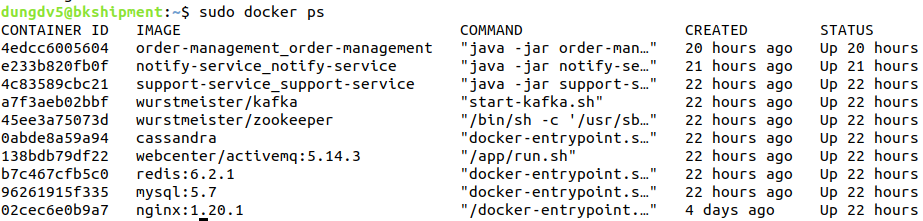
\includegraphics[width=0.8\linewidth]{Images/DockerResult}
		  	\linebreak
		  	\caption{Kết quả}
		  \end{figure}
	  
	  \newpage
	  
	  \section{Bài toán bảo mật các service trong private network, cấu hình SSL, cân bằng tải}
	  
	  
	  Thông thường sau khi deploy thì các service được gọi thống qua \textbf{IP:port/service-name/...}, điều này có nghĩa là service sẽ được public ra bên ngoài. Điều này có thê gặp một số rủi ro về vấn đề an ninh và bảo mật. Vì thế nhóm đã sử dụng NGINX như là một \textbf{Reverse Proxy} để tăng cường bảo mật, cũng như cân bằng tải.
	  
	  
	  \begin{figure}
	  	\centering
	  	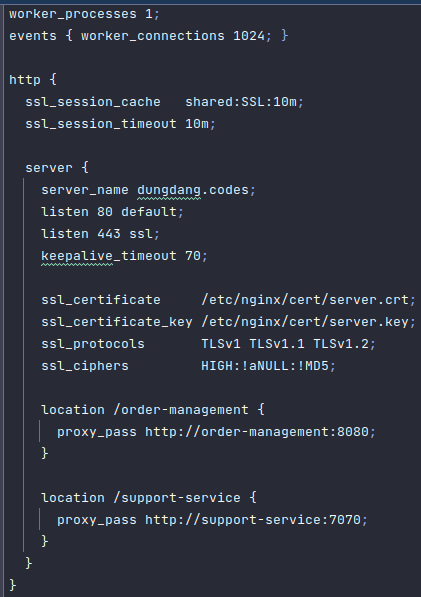
\includegraphics[width=0.8\linewidth]{Images/NGINXconfig}
	  	\linebreak
	  	\caption{Cấu hình của NGINX}
	  \end{figure}
  
  		
  
  
  	
		Như trên file đã cấu hình thì server Frond end có thể gửi request xuống server Back end thông qua domain là: \textbf{dungdang.codes} ở port 80 cho HTTP và 443 cho HTTPS. Đối với những request có domain là: https://dungdang.codes/order-management/... sẽ được route vào service đươc deploy ở port 8080 còn https://dungdang.codes/support-service/... thì sẽ được route vào service deploy ở port 7070
		
		Điều này đã giúp che giấu và bảo mật các services chạy trong private network.
		
		\newpage
		
		
		  
		  
		  

		    
		  
